\chapter{Physical Modelling of Musical Instruments}\label{ch:physMod}
At the time of writing, an uncountable number of digital musical instruments exists. This range encompasses both digital keyboards that can create sounds from various real (and non-real) instruments, as well as digital instrument plug-ins used by music producers in Digital Audio Workstations (DAWs). Many of these digital instruments are based on samples, or recordings, of their real-life counterparts, while others use computationally cheap methods to generate sounds, some inspired by physical musical instruments. \todo{add wavetable synthesis}In the 1960s, for example, efficient sinusoidal-based and filter-based sound synthesis techniques such as additive synthesis, subtractive synthesis, or FM (frequency modulation) synthesis  were invented \cite{Roads1996, Chowning1973}. The latter became widely popular through the Yamaha DX7 synthesiser created in 1983 that synthesised sounds based solely on this technique \cite{DX7}. Through a simple change of variables, FM synthesis can generate sounds ranging from brass instruments to drums. 

These techniques are referred to as \textit{spectral modelling} methods, where the manipulation of sinusoids or filtering noise would produce (harmonic) sounds, that could be perceived by the listener as originating from a physical instrument. This top-down approach which starts at the perception of the listener, has advantages in terms of computational efficiency, but is quite limited by the systems it can model \cite{Smith2010a}. 

As computing power increased over the last few decades, using \textit{physical models} rather than samples or spectral modelling methods gained an increased popularity.
Physical modelling, in the context of sound and music, is a way to generate sound based on physical processes, including string vibrations in a guitar, air propagation in a trumpet, or even the reflections in a concert hall. When compared to spectral modelling, this is a bottom-up approach that attempts to model the sound from the source.  

This work focuses on simulating\footnote{The term \textit{emulated} is only used in the title of this work (because of the alliteration), but is synonymous to \textit{simulated} in this context.} traditional musical instruments using physical modelling. 
The interest in physically modelling traditional musical instruments is twofold: 1) sound generation, and 2)understanding of the underlying physical processes, the former being main focus of this PhD project. One of the reasons why one would use physical models rather than samples of the real instrument, is that a model is much more flexible to player control. Consider the violin as an example, where the performer controls the bow force, velocity and position along the string, as well as the finger determining the pitch of the string. A physical model can generate the sound in real time based on these performance parameters. If samples were to be used, every single combination of these parameters would need to be recorded in order to capture the entire instrument.\todo{add note on violin recording listen to 20k cremona podcast}
A more in-depth reasoning behind using physical models for sound generation will be given in Section \ref{sec:why}.

This chapter continues by giving a brief overview of the history of physical modelling for sound synthesis.

\section{A Brief History}\label{sec:history}


% As computing power increased, so did the popularity of using physics-based simulations of musical instruments. 
Most likely the very first example of a physically modelled musical sound is the ``Bicycle Built for Two'' by Kelly, Lochbaum, and Matthews in 1961\footnote{\url{http://ccrma.stanford.edu/~jos/wav/daisy-klm.wav}}. It uses what later got known as the Kelly-Lochbaum vocal-tract model to generate a voice and was published the year thereafter \cite{Kelly1962}. 

The very first musical instrument simulations were based on discretisation of differential equations using \textit{finite-difference time-domain} (FDTD) methods. These were carried out around 1970 by Hiller and Ruiz \cite{Ruiz1969, Hiller1971I, Hiller1971II} and applied to the wave equation to simulate string sounds. The sound generation, however, was far from real-time and it took several minutes to generate only $1$ second of sound. In 1983, Cadoz et al. introduced CORDIS, a real-time sound generating system based on \textit{mass-spring networks} \cite{Cadoz1983}.
The first physical model of the bowed string was due to McIntyre et al. in their 1983 publication \cite{McIntyre1983}. In the same year Karplus and Strong devised an extremely efficient way to generate a string sound in \cite{Karplus1983} later known as the Karplus-Strong algorithm. Based on these ideas, Smith coined the term \textit{digital waveguides} around the late 1980s and early 1990s in \cite{Smith1987, Smith1992} and continued to develop the method \cite{Smith2010b}.
Around the same time, Adrien in \cite{Adrien1991} and later Morrison and Adrien in \cite{Morrison1993} introduced \textit{modal synthesis}, a way to synthesise an object's sound by decomposing it into its modes of vibration. 

Although more techniques have been developed in the last 20-30 years, most of the developments in the field of physical modelling for musical instruments are based on those presented in this section. Before moving on to further details about these methods in Section \ref{sec:physModTech}, a modular approach to subdivide a musical instrument will be presented.

\section{Exciter-Resonator Approach}\label{sec:exciterResonator}
Nearly any musical instrument can be subdivided into a resonator component and an exciter component, both of which can be simulated individually. This modular approach to musical instruments was first introduced by Borin, De Poli and Sarti in \cite{Borin1989} and and later developed by De Poli and Rocchesso in \cite{Poli1998} and is used to structure this work. Examples or resonator-exciter combinations are the violin and the bow, or the trumpet and the lips of the player. %\SWcomment[Note that Part \ref{part:interactions} does not include the interactions between the resonator and exciter, but rather the interactions between different parts of the resonator itself, for example, the interactions between the string and the body of a violin, which both are resonators.]

A resonator is a passive system, in this work mostly assumed to be linear, and does not emit sound unless triggered by an external source. Exciters can be seen as these external sources, and generally have a nonlinear element.\footnote{The difference between linear and non-linear systems is in their response to input level or amplitude. The behaviour of linear systems does not change with the level of the input. Instead, it only scales (linearly) with the input level, i.e., an input to a linear system with twice the amplitude yields an output of twice the amplitude. The behaviour of nonlinear systems, however, does change depending on the level of the input. Although linear systems are rarely found in the real world, under low amplitude excitations most systems can still be considered linear and their nonlinear effects can be ignored.} Exciters insert energy into a resonator and cause it to vibrate and emit sound, and the method of excitation greatly influences the sound of the resonator. In the real world, the interaction between the exciter and the resonator is bi-directional. In other words, the exciter not only affects the state of the resonator, but the resonator affects the exciter as well. For the most part, this is also what is attempted to model in this work.

The next section will talk about various techniques that can be used to implement the resonator. Details on  excitation modelling are left for Part \ref{part:exciters}.

\section{Physical Modelling Techniques}\label{sec:physModTech}
The time-evolution of dynamic systems, including that of musical instruments, can be well described by partial differential equations (PDEs) \cite{Fletcher1998, theBible}. Examples of a dynamic systems are a guitar string, a drum-membrane, or air propagation in a concert hall; three very different concepts, but all based on the same types of equations of motion. Many of these equations and other knowledge currently available on the physics of musical instruments have been collected by Fletcher and Rossing in \cite{Fletcher1998}. Though these equations are very powerful, only few have a closed-form solution, and in order for them to be implemented, they need to be approximated. In the past decades, much research has been done on implementing these PDEs to model and simulate different musical instruments. Great overviews of implementation techniques are given by, for example, Vesa V{\"a}lim{\"a}ki et al. in \cite{Valimaki2006} and Julius O. Smith in \cite{Smith2010a, Smith2010b}. 
\\

The most popular physical modelling techniques that are described in this literature can be found below:
\\
\\
\textit{Modal Synthesis} decomposes a system into a series of uncoupled `modes of vibration' and can be seen as a physically-based additive synthesis technique. First used in a musical context by Morrison and Adrien in \cite{Morrison1993}, it is a technique that is still used today due to its computational efficiency, especially when simulating higher-dimensional systems such as (two-dimensional) plates or (three-dimensional) rooms. It is especially effective when used to describe a linear system with a small number of long-resonating modes \cite{Bilbao2018, Smith2010a}. When used to describe nonlinear systems, however, the modes become `coupled’ and the system will quickly become more computationally expensive. Recent developments using the FAUST programming language allow a 3D-mesh model of any three-dimensional object to directly be decomposed into its modes of vibration and used as a sound-generating physical model \cite{MichonMesh2Faust2017}.
\\
\\
\textit{Finite-Difference Time Domain} methods (FDTD) aim to solve PDEs by approximating them with difference equations, discretising a continuous system into grid-points in space and time. In a musical context, this technique was first used for the case of string vibration by Hiller and Ruiz in \cite{Ruiz1969, Hiller1971I, Hiller1971II} and later by Chaigne in \cite{Chaigne1992, Chaigne1994}. Bilbao extensively describes this method in \cite{theBible, Bilbao2018}. Although computationally expensive, especially when working with higher-dimensional systems, this technique could potentially accurately model any system, whether it is linear or nonlinear, time-invariant or time-variant.
\\
\\
\textit{Digital Waveguide Modelling} (or Digital Waveguides (DWGs)) is a technique that discretises wave propagation and scattering. The technique was first presented by Smith in \cite{Smith1987, Smith1992}, and is mostly used for one-dimensional systems, such as strings and acoustic tubes and decomposes their system into travelling wave components. This technique has also been used in higher-dimensional systems, but is superior in efficiency when used in the one-dimensional case \cite{Valimaki2006}. Some authors have combined DWGs with FDTD methods (such as in \cite{Erkut2002, Maestre2014}) to accurately model nonlinear behaviour while maintaining high-speed implementation.
\\
\\
\textit{Mass-spring networks} can be similar in nature to FDTD methods, but treat each grid point as an individual mass connected to other masses through springs in a network. Pioneered in a musical context by Cadoz in \cite{Cadoz1979, Cadoz1983, Cadoz1993} it is currently being further developed by Leonard and Villeneuve in a real-time, interactive environment \cite{Villeneuve2019, Leonard2019}.

\subsubsection{Discussion}
This work focuses on physical modelling using FDTD methods. The main advantage of these methods is that they are extremely general and flexible in terms of the types and number of systems they can model. They allow any set of PDEs to be directly numerically simulated without making any assumptions regarding travelling wave solutions or modes. Moreover, FDTD methods allow for various PDEs, fx. a violin body and four strings, to be connected in a fairly straightforward manner. DWGs, for example, assume a travelling wave solution, which makes complex nonlinear effects extremely hard to model using this technique. To use modal synthesis for modelling a PDE, it requires the system to have closed-form or analytical solution. If this is not available, (finite-element) analysis of the system could be performed to obtain the modal shapes and frequencies of the system. This in itself is very computationally expensive and requires a lot of storage if the modal data needs to be saved. 
\todo{check all of this}
 
The main drawback of FDTD methods is the fact that they require great attention to numerical stability of the solution \cite{theBible}. For a wrong choice of parameters, the implemented system could become unstable and ``explode''\footnote{I learned the hard way that one should always implement a limiter when working with real-time physical models to avoid dangerously loud sounds.}. Stability analysis as well as energy analysis techniques are invaluable in the process of ensuring a stable implementation and much attention to this will be given throughout this work.

A final drawback of using FDTD methods is that -- especially for higher-dimensional systems -- they are much more computationally heavy than other methods, such as DWGs or modal synthesis techniques. The bright side -- if one believes in Moore's law \cite{Moore1965} -- is that it can be assumed that computing power will continue to increase and that within several years, running high-quality simulations of musical instruments based on FDTD methods in real time, will not be an issue.

\section{Applications of Physical Modelling}\label{sec:why}
So why would we go through all this hassle of modelling musical instruments? Could we not use a recording of the original instrument and play that back at the right moment? Or taking another step back, why not buy a real instrument and learn to play that instead? This section aims to answer those questions, by providing some applications of physical modelling for musical instrument simulations. \SWcomment[Very informal section, but I kinda like it :)]

\subsection{Samples vs. Physical Modelling}
%First of all, physical modelling can be used to generate sound in audio plug-ins or digital instrument controllers (such as keyboards). 
Despite the existence of many techniques to simulate musical instruments mentioned in the previous section, the bulk of the currently available digital musical instruments are still based on samples. This is mainly due to the computational power needed to generate sounds as opposed to simple playback of recordings. Furthermore, digital musical instruments based on samples, have an optimally realistic sound. As the output of the digitised instrument is exactly that of the original instrument, the digital version should thus sound indistinguishable from the original.

That said, it can be argued that these are the only advantages of using samples over physical models in this context. Samples are static and unable to adapt to changes in performance; the recording is made by one player with one playing style or technique, using one specific microphone to record the sample, etc. Even if one accepts this, capturing the the entire interaction space of an instrument is nearly impossible. Imagine recording a violin with every single combination of bowing force, velocity, position, duration and other aspects such as vibrato, pizzicato. Even if a complete sample library could be created, this would contain an immense amount of data and take an incredible amount of time to record. 

Using physical models to simulate the musical instrument instead, allows the sound to be generated on the spot based on all the aforementioned interaction parameters. One is not stuck to a single recording of the instrument and, given the right tools or controller, one can alter the sound just as one can with its real-life counterpart.

A drawback of physical models is that, in order to generate a realistic sound, a highly accurate physical description of the original instrument is needed. Apart from (potentially) taking a lot of time to develop this model and tuning its parameters, the eventual implementation will be (much) more computationally expensive than if samples were to be used. Generally, the more accurate the model is, and thus the more true the sound is to the original, the higher the computational cost becomes. 

The main trade-off between samples and physical models is thus storage versus speed, or hard-disk versus CPU. Whether one method should be used over the other depends on the situation. If efficiency is required and the lack of flexibility in the sound is not an issue, samples might be the better choice. If, on the other hand, one wants to create a full digital version of a traditional instrument that responds to player-interaction in the same way as the original instrument would, a physical model should be chosen instead.

\subsection{Resurrect Old or Rare Instruments}
% Why not use the real instrument in the first place? 
Many instruments exist that are too old, too rare, or too valuable to be played. Some live behind museum glass only to be looked at by visitors, never to be played again. In these cases, it might even be hard to record samples of the musical instrument. If, however, the physics (geometry and material properties) of the instrument are available, a physical model of the instrument could be created and its sound brought back too life.

However, applications of physical modelling are not limited to old or rare instruments. Popular musical instruments also require maintenance and might need to be replaced after years of usage. A simulation of these instruments will not age, unless that is of course desired and included in the model.

\subsection{Go Beyond what is Physically Possible}\label{sec:impossible}
As a digital simulation is not restricted by the laws of physics of the real world, this opens up a substantial amount of possibilities.
Musical instrument simulations make it possible for parameters like shape, size, material properties, etc. to be dynamically changed, which is physically impossible or very hard to do. A physical model of a violin could potentially change size and `morph' into a cello while the simulation is running and a player is interacting with it. New ways of interaction and expression could be devised that control the physics of the instrument, expanding the range of possibilities for the musician. 

Furthermore, different instrument components can be combined to create hybrid instruments. For example, one could bow the air in a trumpet, or lip-excite a string (similar to what Smith states in \cite{Smith2010a}). This could potentially result in unique sounds that can only be created using physical models.

\section{Project Objectives and Main Contributions}
This section presents several research questions and provides the main objectives and contributions of the project. 

\subsubsection{How can computationally expensive physical models be made playable in real-time?}

The biggest challenge in real-time audio applications, as opposed to those only involving graphics for example, is that the sample rate required is extremely high. As Nyquist's sampling theory states, a sampling rate of at least 40 kHz is necessary to produce frequencies up to the human hearing limit of 20 kHz \cite{Nyquist}. Most graphics applications are made with a temporal sample rate (mostly referred to as frames per second (FPS)) of around 60 Hz \cite{Yantis2016}, which is orders of magnitude smaller than the auditory sample rate.\todo{Look at this}

Even though physical modelling has been a popular research field in the past few decades, relatively little research has been done on making the models work in real-time, i.e., `playable’ \cite{Mehes2016}. Several virtual string instruments and different electric pianos have been made real-time by Pfeifle and Bader in \cite{Pfeifle2012, Pfeifle2015, Pfeifle2017}. The authors used field programmable gate arrays (FPGAs) for implementing models based on FDTD methods. Furthermore, Roland’s V-series use COSM (Composite Object Sound Modelling) technology \cite{Bybee2019} that implement real-time physical models in hardware instruments. In the NESS project, Stefan Bilbao and his team focused on implementing systems using FDTD methods in real-time using parallelisation techniques and the GPU \cite{Bilbao2019CMJa,Bilbao2019CMJb}. 

The main objective of this work is to implement physical models simulated using FDTD methods in real time without the need of special hardware, i.e., on a regular personal computer or laptop. The objective is not to renew the underlying models themselves, but novel combinations were be made to simulate relatively unknown instruments as test cases for this objective. The instruments modelled over the course of this project are the esraj (Bowed Sitar), hammered dulcimer and hurdy gurdy presented in paper \citeP[A], the tromba marina presented in paper \citeP[D] and the trombone presented in paper \citeP[H], all implemented in real time using FDTD methods. An extended summary of these papers can be found in Part \ref{part:contributions}.

\subsubsection{How can (the sound of) traditional instruments be extended upon?}
As mentioned in Section \ref{sec:impossible}, using physical modelling to simulate real-life instruments relieves the physical limitations that the real world imposes on them.
As FDTD methods are quite rigid, dynamically changing parameters while the instrument simulation is running, is a challenge. Other techniques, such as modal synthesis, are much more suitable for this, but come with the drawbacks mentioned in Section \ref{sec:physModTech}. Therefore, one of the main objectives of this project was to devise a method to allow parameters in musical instrument simulations based on FDTD methods to be dynamically varied.

Indeed, during this PhD project, a novel method was devised to smoothly change parameters over time, introducing this to FDTD methods. This method was published in \citeP[G] and will be elaborated on in Chapter \ref{ch:dynamicGrid}.

\subsubsection{How can the now-virtual instruments be controlled in a natural way?}

A great challenge in musical instrument simulations is their control. In many physical instruments, one interacts immediately with the sound-creating object, such as a string on a guitar or a membrane on a drum. This allows the musician to be much more expressive than if they only used the keyboard and mouse. 
Expressivity, however, is not the only thing that makes an instrument interesting and enjoyable to play. The interaction with a musical instrument simulations could feel very `dry' or unnatural as there is no haptic feedback; something present in (nearly) all physical musical instruments. 

The last objective of this PhD project is thus to find ways to control the instrument simulations in an expressive way. 
Over the course of this PhD project, the Sensel Morph, or Sensel for short, has been used extensively  \cite{sensel}. The Sensel is a controller containing ca. 20,000 pressure sensors in a small area that allow for highly expressive control of the instruments. This controller has been used in papers \citeP[A], \citeP[B], \citeP[C] and \citeP[D].

Although the Sensel allows for more expressive control than a keyboard and mouse, it does not resemble any of the interaction paradigms of the original instruments. It was thus attempted to include a controller that would be more suited for controlling the musical instrument simulation and allow for a more intuitive control.
For one of the projects, described in paper \citeP[E], a virtual-reality implementation of the tromba marina is controlled by the PHANTOM Omni \cite{phantom} which is a six-degrees-of-freedom haptic device. The controller contains a hand-held pen-like object that is attached to a robotic arm and can be linked to a virtual environment to provide force and vibrotactile feedback through the arm based on this environment. 

\section{Thesis Outline} 
\SWcomment[not done: ]Although a collection of papers format has been used for the structure of this thesis, the introductory part to the papers has been written in a monographic style. This hybrid format  

This thesis is divided into several parts which in their turn are divided in chapters. See Figure \ref{fig:thesisOutline} for a visual overview of the thesis structure. 

\subsubsection{Part \ref{part:introduction}: Introduction}
This part introduced the field of physical modelling for musical instruments here in Chapter \ref{ch:physMod} by giving a brief history of the field and providing and background for the project. Furthermore, the project objectives and contributions to the field have been detailed. Chapter \ref{ch:FDTD} will provide a thorough introduction to finite-difference time-domain methods using simple sound-generating systems as examples, after which Chapter \ref{ch:analysis} will introduce several analysis techniques in a tutorial-like fashion.

\subsubsection{Part \ref{part:resonators}: Resonators}
The resonator component of a musical instrument, as introduced in Section \ref{sec:exciterResonator}, can -- for most instruments -- be further decomposed into more basic resonators. In order to model the violin, for example, one can decompose the entire resonator into four strings and its body. Chapter \ref{ch:stiffString} will present a model for the stiff string, Chapter \ref{ch:brass} will introduce acoustic tubes that can be used to model brass instruments and Chapter \ref{ch:2Dsyst} will introduce two-dimensional systems such as membranes and plates which can be used to simulate simplified instrument bodies.

\subsubsection{Part \ref{part:exciters}: Exciters} 
As stated in Section \ref{sec:exciterResonator} stated, the excitation greatly determines the behaviour of the resonator. This pert
presents various ways in which the resonators introduced in Part \ref{part:resonators} can be excited. Chapter \ref{ch:physInspExcitations} introduces `physically inspired' excitations, Chapter \ref{ch:bow} introduces the bow and presents the contribution made in paper \citeP[C], and finally, Chapter \ref{ch:lipreed} presents the lip reed used to excite brass instruments.

\subsubsection{Part \ref{part:interactions}: Interactions}
As mentioned before, most musical instruments consist of many individual resonators, and to properly model these, their interaction must be taken into account. This part two different ways that the resonators can interact with each other; collisions between various resonators are presented in Chapter \ref{ch:collisions} and connections between them in Chapter \ref{ch:connections}. 
\\
\\

\noindent The above parts are used as an introduction for the main contributions of the PhD project and -- with the exception of Chapter \ref{ch:bow} -- do not contain any novelty. Much effort has been put in explaining the existing methods and models from the literature used in this project in a way that is slightly more in-depth and pedagogical than might be common for a PhD thesis (specifically Part \ref{part:introduction}). It is the hope of the PhD student that going this extra mile could make this work (and the above parts in particular) be a contribution in itself: to put this research field into reach of beginners in the field of physical modelling for sound synthesis using FDTD methods without the need of much experience in the fields of physics, mathematics or computer science. 
\\

\subsubsection{Part \ref{part:contributions}: Contributions} This part contains extended summaries of the main contributions of the PhD project. Chapter \ref{ch:dynamicGrid} summarises paper \citeP[G] and extends it by providing some design considerations. Chapter \ref{ch:realtime} explains the considerations necessary for real-time implementation of physical models. Chapters \ref{ch:largeScale}, \ref{ch:tromba} and \ref{ch:trombone}, summarise papers \citeP[A], \citeP[D] and \citeP[H] respectively and extend the papers mainly with more implementation details.

\subsubsection{Part \ref{part:conclusion}: Conclusions and Perspectives}
This part concludes the thesis and puts the contributions into context of the physical modelling field. Future perspectives and possible continuations of this work are given as well.
\\

Finally, \textbf{Part \ref{part:papers}: Papers} contains the main publications made over the course of this PhD project and an appendix appears in \textbf{Part \ref{part:appendix}: Appendix}.

\begin{figure}[h]
    \centering
    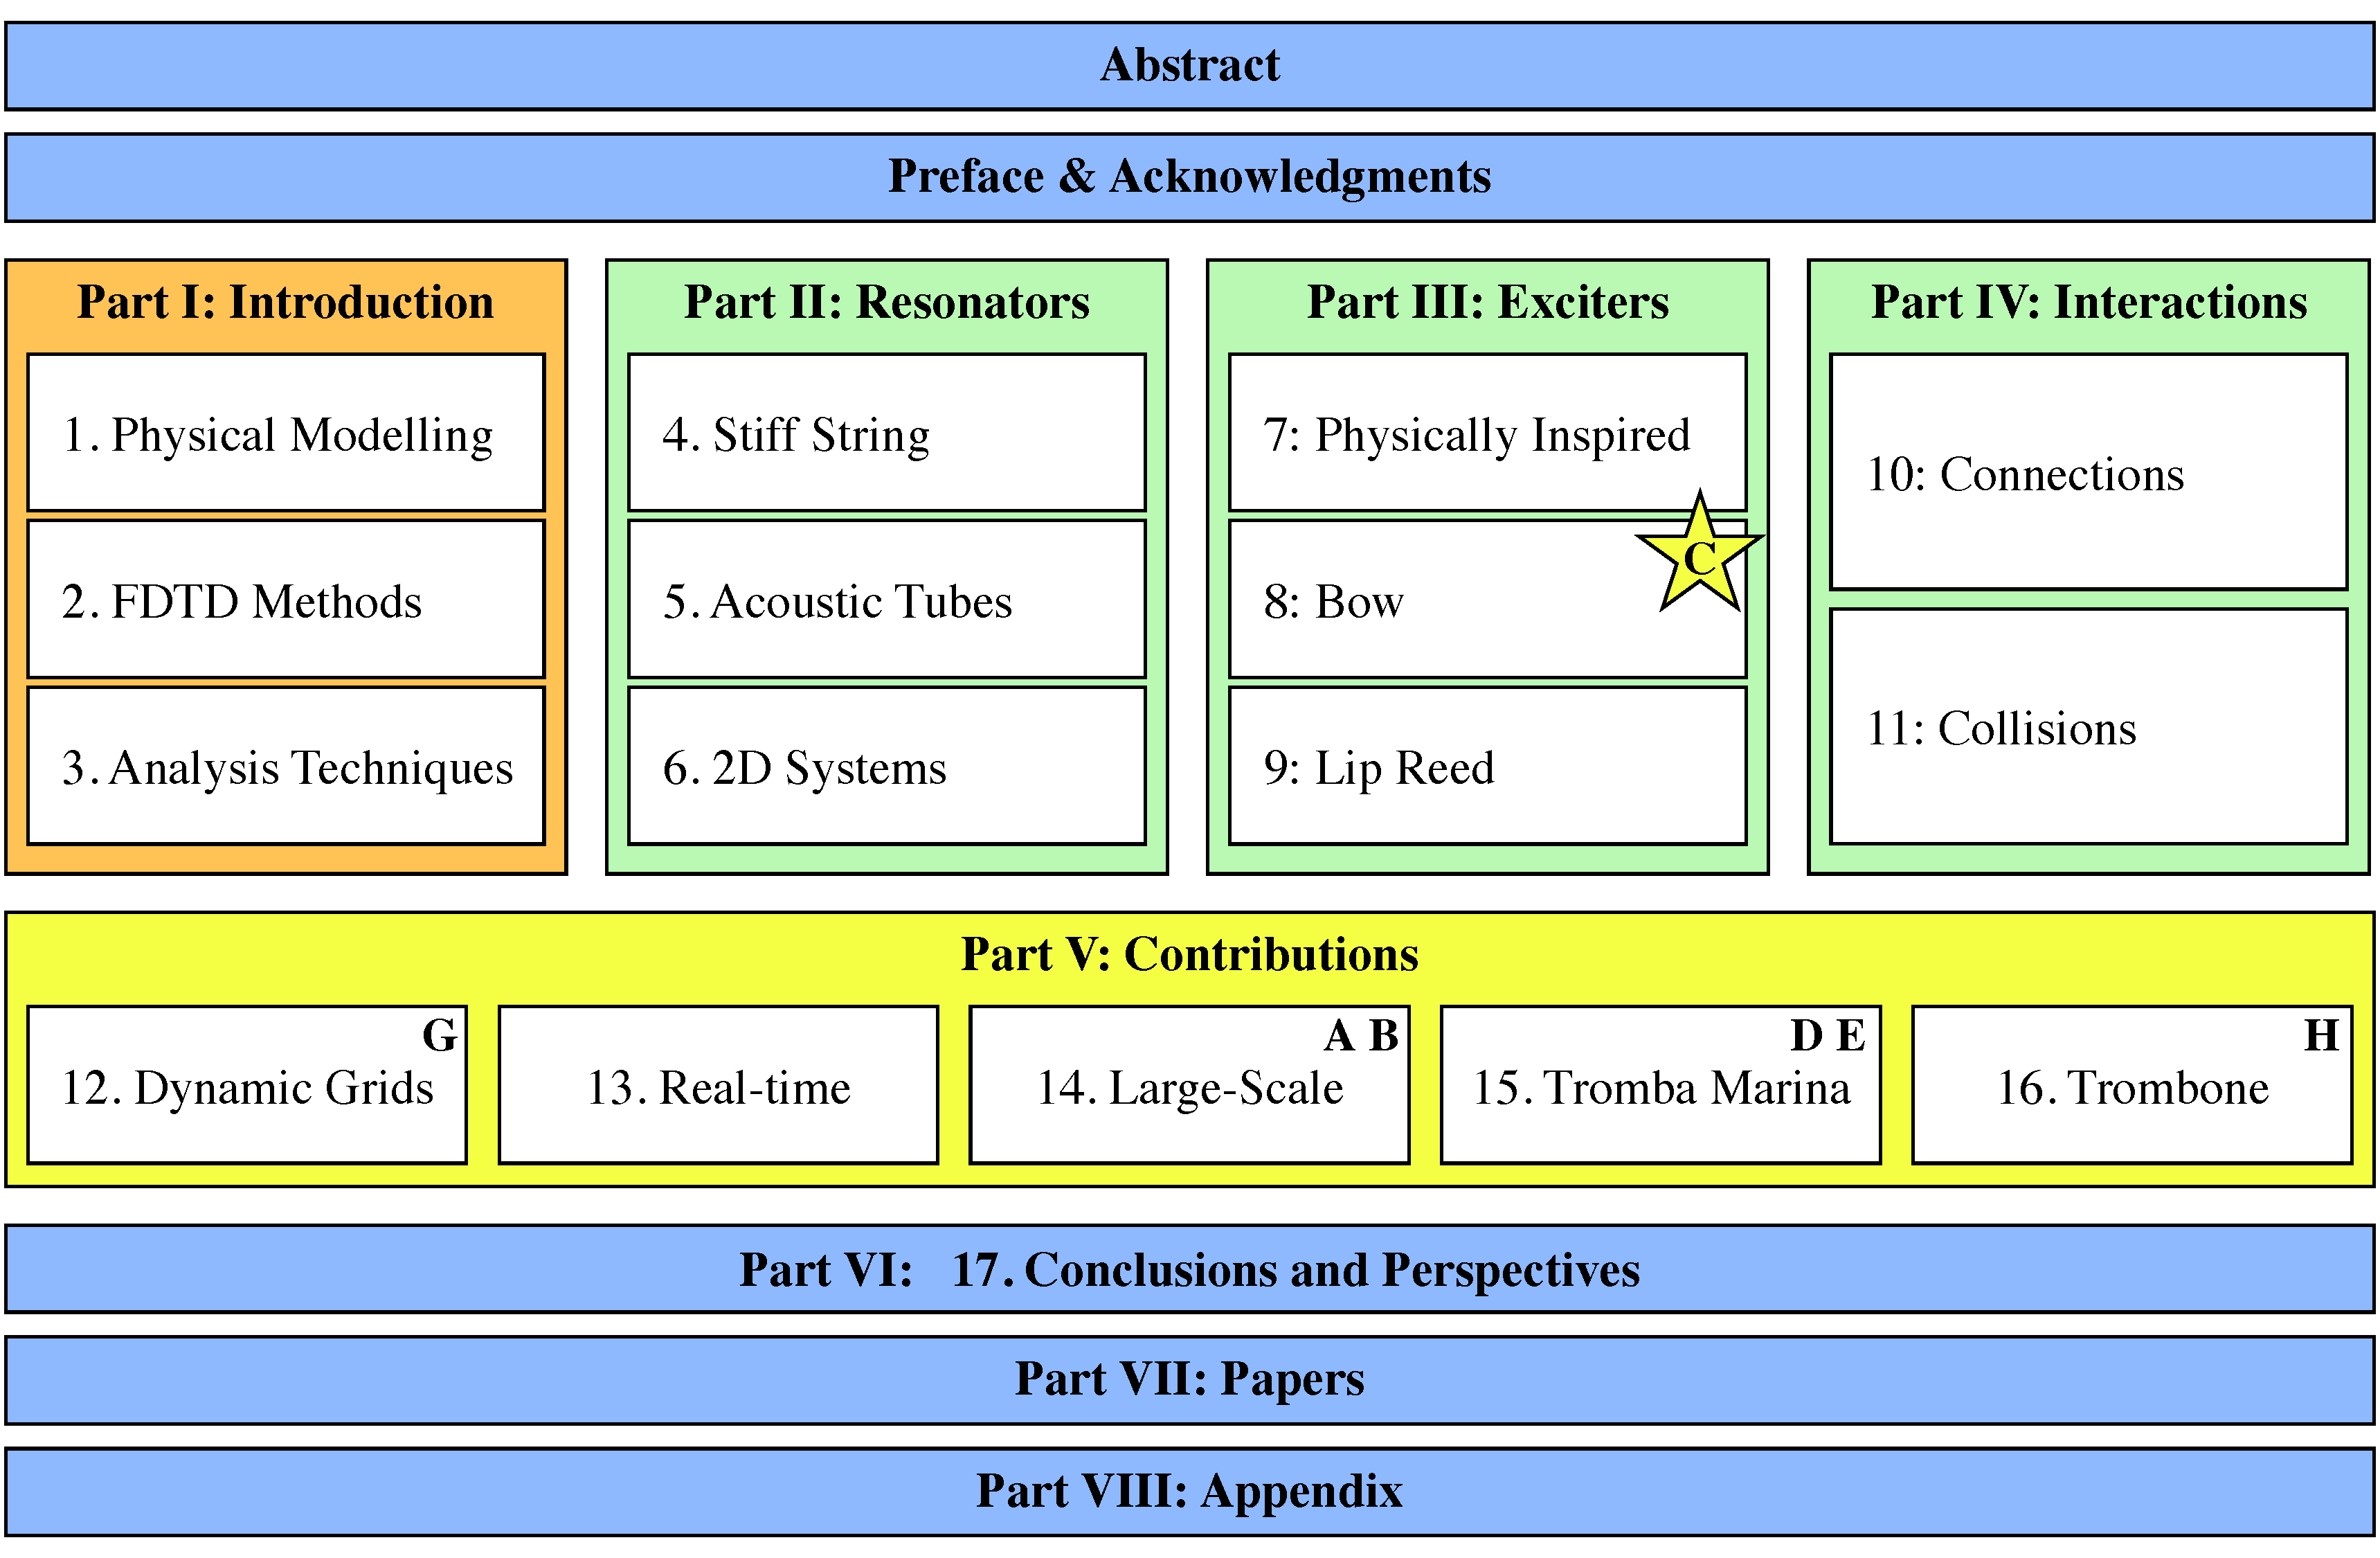
\includegraphics[width=\textwidth]{figures/intro/thesisOverview.pdf}
    \caption{\label{fig:thesisOutline} The outline of this thesis. The contributions made throughout the PhD project are marked in yellow. Most are collected in Part \ref{part:contributions}, though the novel work done on the bow will already appear in Chapter \ref{ch:bow}. Marked in green are the parts that describe the physical models which the contributions are based on. The basics of the methods used for these models are introduced in Part \ref{part:introduction} marked in orange. The chapters that can be seen as an extended summary of the papers in Part \ref{part:papers} are indicated by the letter of the respective paper.}
\end{figure}